
ラジコンの曲がる値を拡大して(大きいハンドル)収集した教師データの学習結果での
自律走行実験も約6回行った.
Fig.\ref{diaRshita}とFig.\ref{diaRshita_270}はニューラルネットワークによる走行と
$b=270,270$の感覚運動写像による
走行の1回の走行実験の時間変化におけるロボット位置の角度($\theta$)と半径($R$)のまとめ図である.
横軸は時間(s),縦軸上のほうが$\theta$,下のほうが$R$である.

この2つグラフから,大きいハンドルでのニューラルネットワークの走行のほうが対面走行を最後まで維持でき,
スムーズに走れると観察された(Fig.\ref{NN300}).
時計回りのロボット達が内側の壁に沿う,反時計回りのロボット達が外側の壁に沿う.

$b=270,270$の感覚運動写像によりの走行のほうが途中に1方交流になった(Fig.\ref{diaRshita_270}.
約250秒からすべての$\theta$の曲線が右に傾斜する),
$R$の変動範囲が大きい(衝突が多い),1方向走行流になったら,$R$の変動も安定になって,
外側の壁に沿って反時計回り走ると観察された(Fig.\ref{SMM300}).


\vspace{-1mm}
\begin{figure}[!ht]
    \centering
    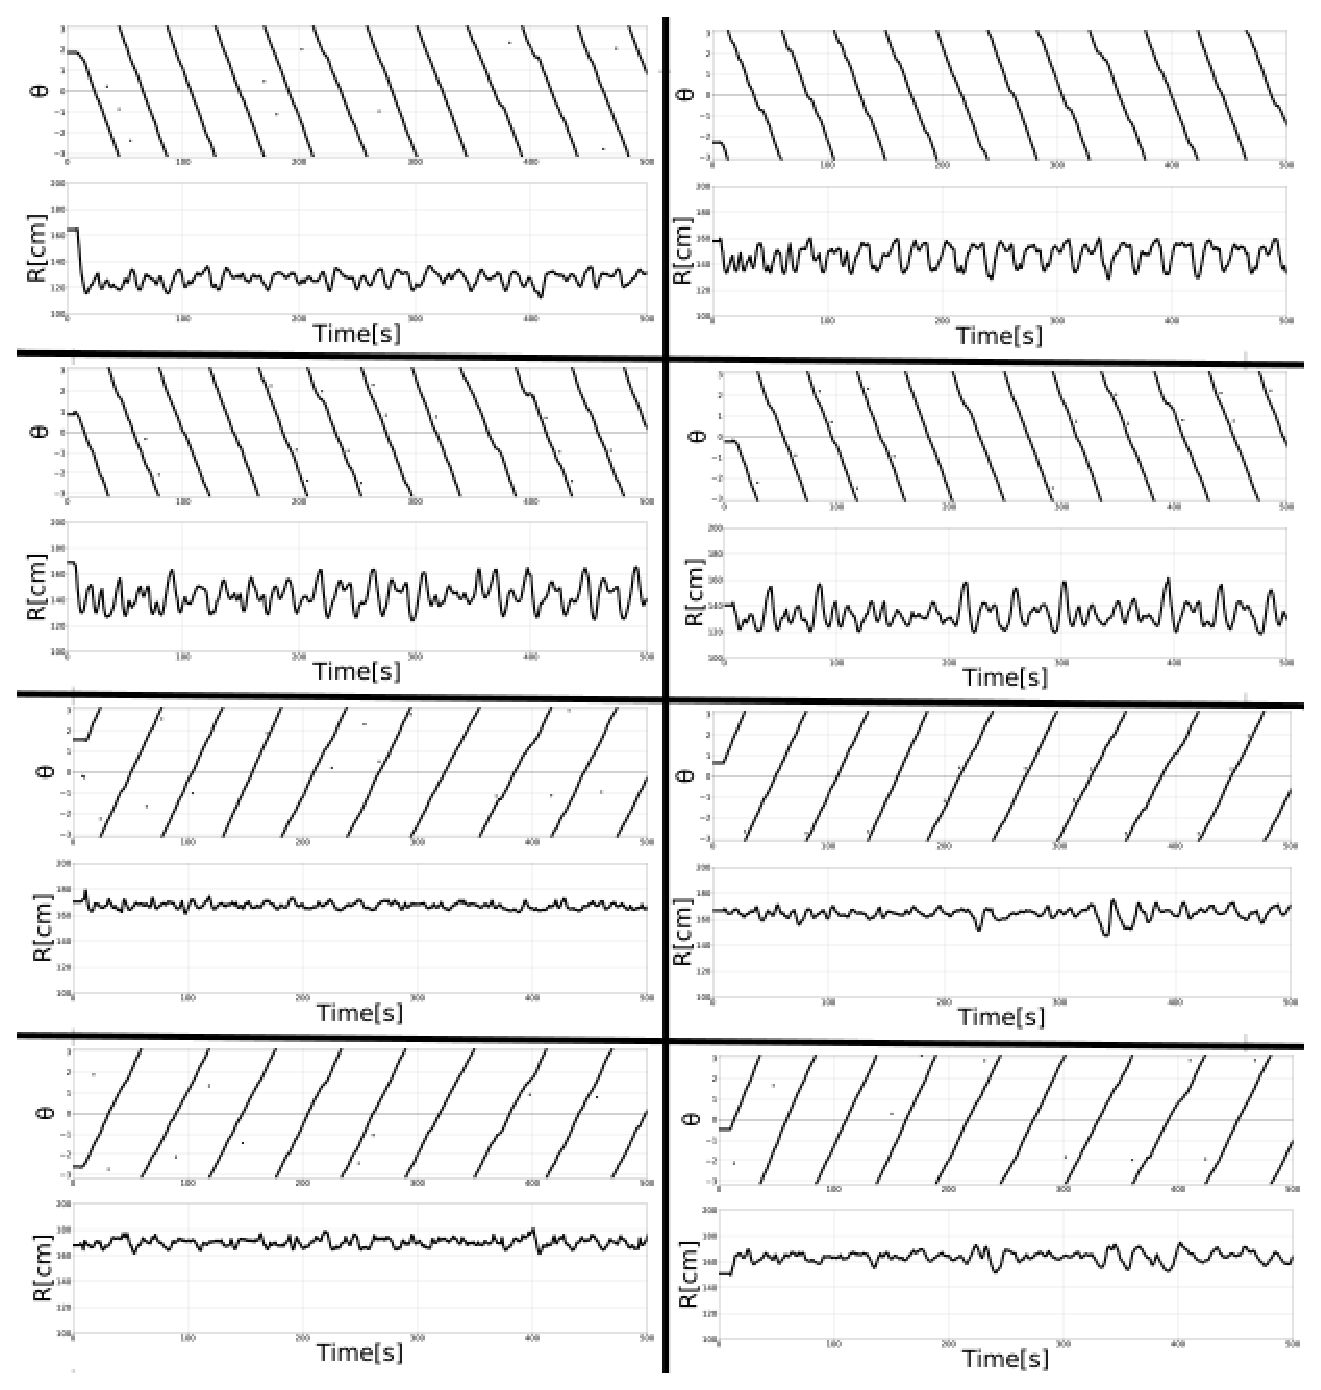
\includegraphics[width=1.0\linewidth]{nn_shita_R_rand.eps}
    \caption{ランダムの初期配置でNNにより走行の$\theta$,$R$と時間の関係図}
    \label{diaRshita}
\end{figure}

\vspace{-4mm}
\begin{figure}[!ht]
    \centering
    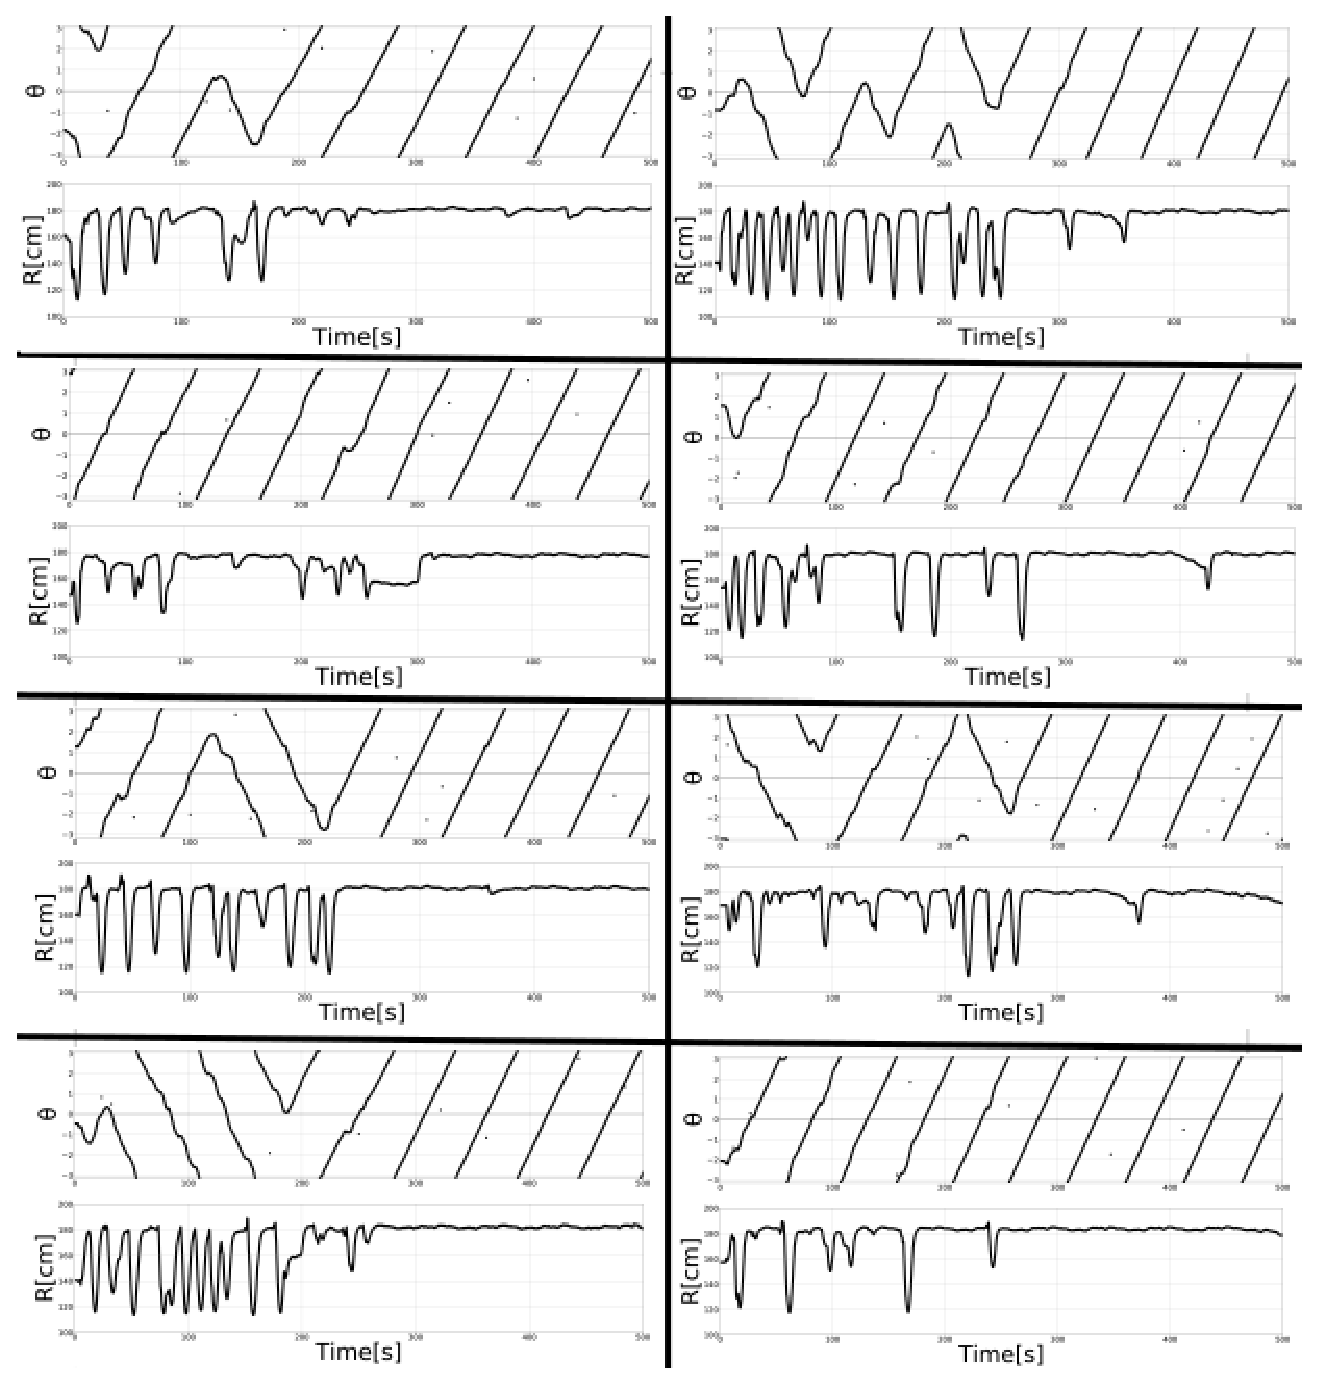
\includegraphics[width=1.0\linewidth]{smm_shita_R_rand270.eps}
    \caption{ランダムの初期配置でSMMにより走行の$\theta$,$R$と時間の関係図}
    \label{diaRshita_270}
\end{figure}

\begin{figure}[h]
    \begin{minipage}{0.48\linewidth}
        \centering
        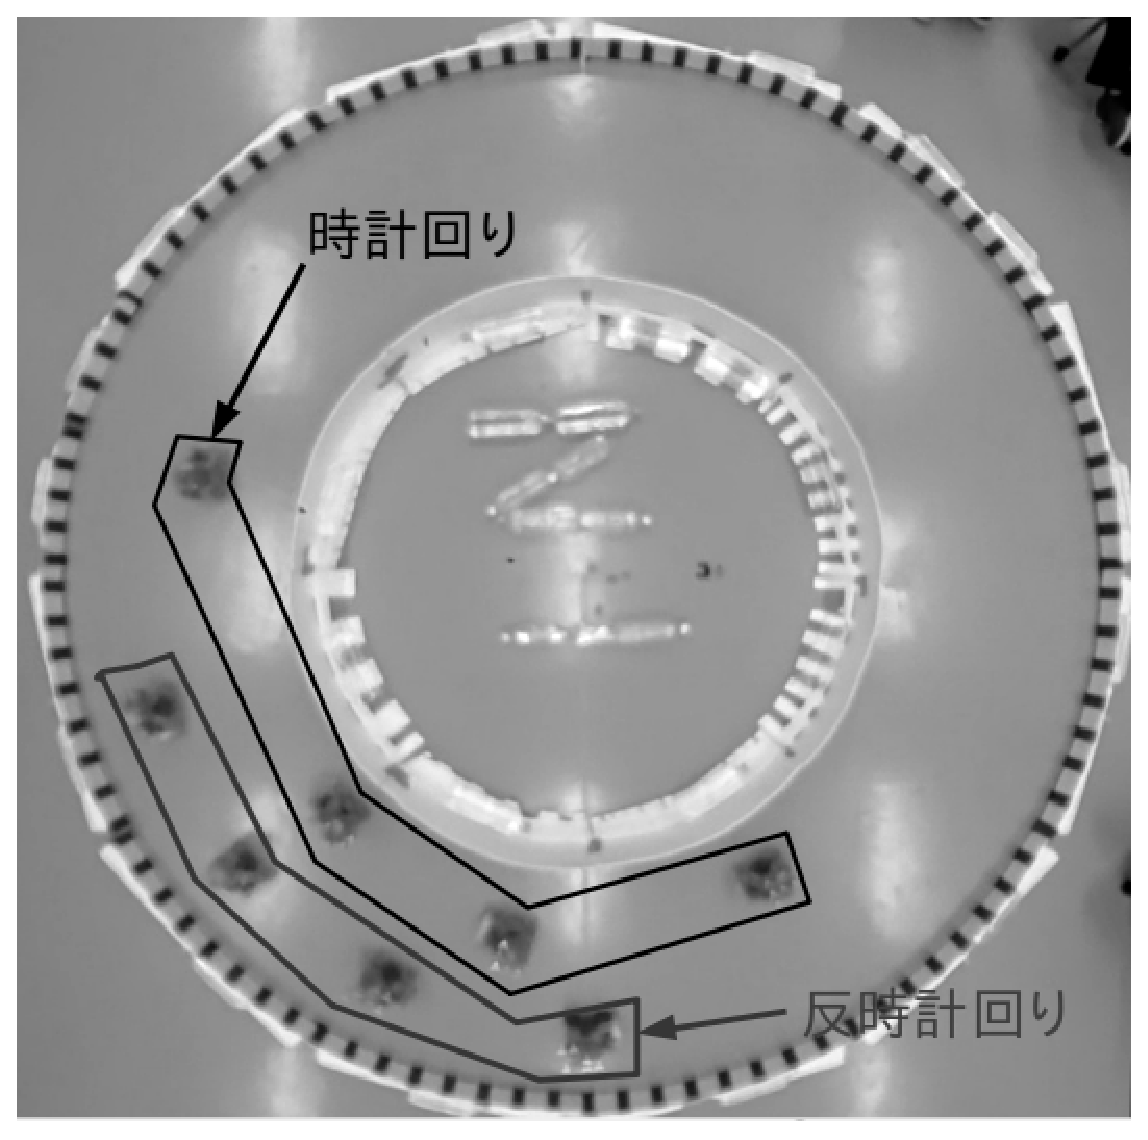
\includegraphics[width=1.0\linewidth]{NN_exp.eps}
        \caption{300秒neural network走行風景}
        \label{NN300}
    \end{minipage}
    \begin{minipage}{0.48\linewidth}
        \centering
        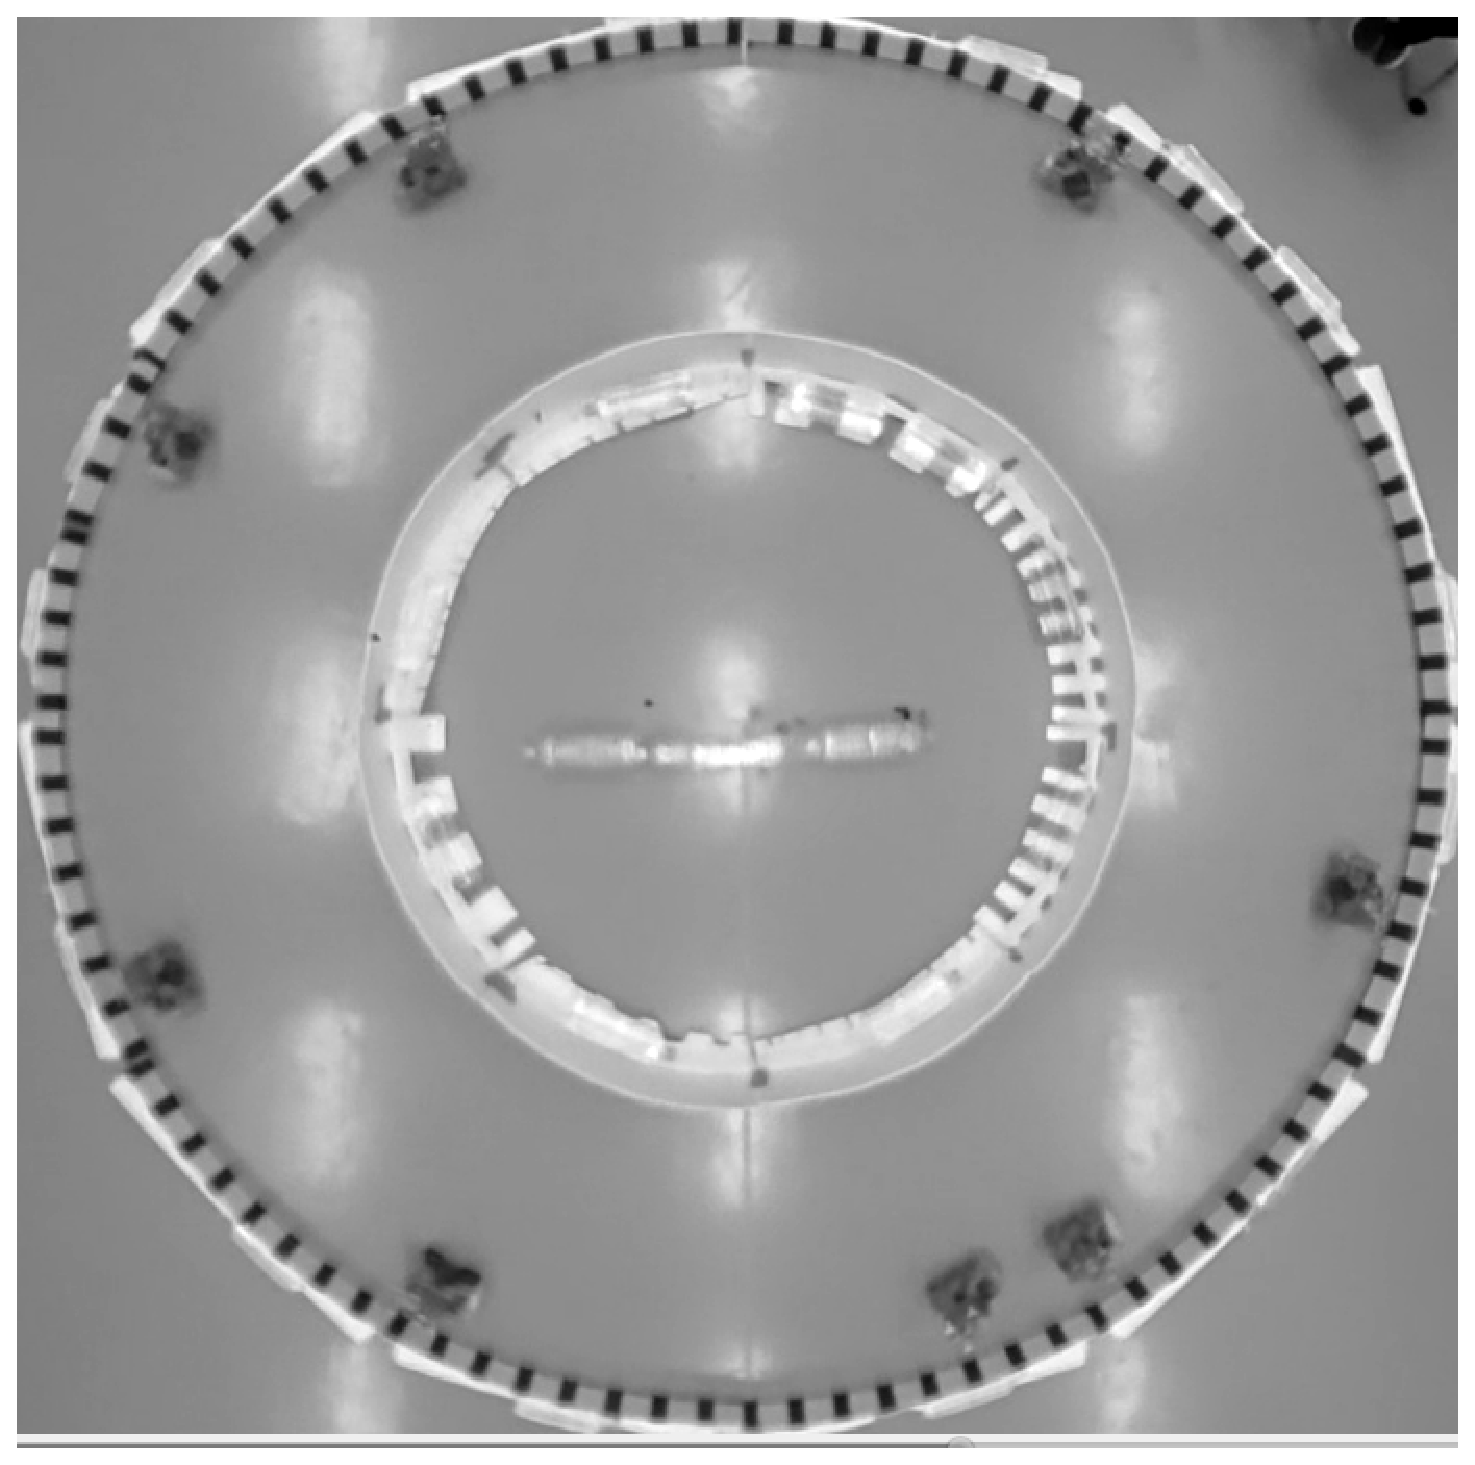
\includegraphics[width=1.0\linewidth]{SMM270_exp.eps}
        \caption{300秒感覚運動写像走行風景}
        \label{SMM300}
    \end{minipage}
\end{figure}
